%!TEX program = xelatex

\documentclass[11pt,titlepage]{report}
%!TEX root = main.tex

\usepackage[T1]{fontenc}
\usepackage{lmodern}
\usepackage[svgnames]{xcolor}
\usepackage{fontspec} % XeLaTeX required!
\usepackage{graphicx}
\usepackage{circuitikz}
\usepackage{tikz}
\usepackage{pifont}
\usepackage[some]{background}
\usepackage{xltxtra} 
\usepackage{setspace}
\usepackage[absolute]{textpos}
\usepackage[latin1]{inputenc}
\usepackage[english]{babel}
\usepackage{graphicx}
\usepackage{wrapfig}
\usepackage{fullpage}
\usepackage[margin=1in]{geometry}
\usepackage{float}
\usepackage{url}
\usepackage{multicol}
\usepackage{hyperref}
\usepackage{titlepic}
\usepackage{standalone}
\usepackage{siunitx}
\usepackage{booktabs}
\usepackage{amsmath}
\usepackage{unicode-math}
\usepackage{verbatim}
\usepackage{enumitem}
\usepackage{listings}
\usepackage{multirow}
\usepackage{pgfplots}
\pgfplotsset{compat=1.8}
\usepackage{caption} 
\usepackage[parfill]{parskip}
\usepackage{import}
\usepackage[backend=bibtexu,texencoding=utf8,bibencoding=utf8,style=ieee,sortlocale=en_GB,language=auto]{biblatex}
\usepackage[strict,autostyle]{csquotes}
\usepackage[final]{pdfpages}
\usepackage{subcaption}
\usepackage{ifplatform}
%\captionsetup[table]{skip=10pt}


% Fix for includepdf bug in Mac OS X
\newcommand{\insertpdfpath}[1]{
	\ifwindows
	\newcommand{\insertpdf}[2]{\includepdf[pages=##1]{##2}}
	\else
	\newcommand{\insertpdf}[2]{\includepdf[pages=##1]{#1/##2}}
	\fi
}

%set fonts
\setmainfont[Ligatures=TeX]{Myriad Pro}
\setmathfont{Asana Math}
\setmonofont{Lucida Console}

\usepackage{titlesec, color}
\renewcommand{\familydefault}{\sfdefault} %set font family
\renewcommand{\arraystretch}{1.2} %set table vertical spacing
\setlength\parindent{0pt} %no paragraph indent
\hypersetup{ %setup hyperlinks
    colorlinks,
    citecolor=black,
    filecolor=black,
    linkcolor=black,
    urlcolor=black
}

%redesign chapter headings
\definecolor{gray75}{gray}{0.75}
\newcommand{\chapternumber}{\thechapter}
\newcommand{\hsp}{\hspace{20pt}}
\titleformat{\chapter}[hang]{\Huge\bfseries}{\chapternumber\hsp\textcolor{gray75}{|}\hsp}{0pt}{\Huge\bfseries}

%Redefine appendix headers
\renewcommand{\appendixname}{Appendix}
\renewcommand{\appendixtocname}{Appendices}
\renewcommand{\appendixpagename}{Appendices}

%For code listings
\definecolor{black}{rgb}{0,0,0}
\definecolor{browntags}{rgb}{0.65,0.1,0.1}
\definecolor{bluestrings}{rgb}{0,0,1}
\definecolor{graycomments}{rgb}{0.4,0.4,0.4}
\definecolor{redkeywords}{rgb}{1,0,0}
\definecolor{bluekeywords}{rgb}{0.13,0.13,0.8}
\definecolor{greencomments}{rgb}{0,0.5,0}
\definecolor{redstrings}{rgb}{0.9,0,0}
\definecolor{purpleidentifiers}{rgb}{0.01,0,0.01}


\lstdefinestyle{csharp}{
language=[Sharp]C,
showspaces=false,
showtabs=false,
breaklines=true,
showstringspaces=false,
breakatwhitespace=true,
escapeinside={(*@}{@*)},
columns=fullflexible,
commentstyle=\color{greencomments},
keywordstyle=\color{bluekeywords}\bfseries,
stringstyle=\color{redstrings},
identifierstyle=\color{purpleidentifiers},
basicstyle=\ttfamily\small}

\lstdefinestyle{c}{
language=C,
showspaces=false,
showtabs=false,
breaklines=true,
showstringspaces=false,
breakatwhitespace=true,
escapeinside={(*@}{@*)},
columns=fullflexible,
commentstyle=\color{greencomments},
keywordstyle=\color{bluekeywords}\bfseries,
stringstyle=\color{redstrings},
identifierstyle=\color{purpleidentifiers},
}

\lstdefinestyle{matlab}{
language=Matlab,
showspaces=false,
showtabs=false,
breaklines=true,
showstringspaces=false,
breakatwhitespace=true,
escapeinside={(*@}{@*)},
columns=fullflexible,
commentstyle=\color{greencomments},
keywordstyle=\color{bluekeywords}\bfseries,
stringstyle=\color{redstrings},
identifierstyle=\color{purpleidentifiers}
}

\lstdefinestyle{vhdl}{
language=VHDL,
showspaces=false,
showtabs=false,
breaklines=true,
showstringspaces=false,
breakatwhitespace=true,
escapeinside={(*@}{@*)},
columns=fullflexible,
commentstyle=\color{greencomments},
keywordstyle=\color{bluekeywords}\bfseries,
stringstyle=\color{redstrings},
identifierstyle=\color{purpleidentifiers}
}

\lstdefinestyle{xaml}{
language=XML,
showspaces=false,
showtabs=false,
breaklines=true,
showstringspaces=false,
breakatwhitespace=true,
escapeinside={(*@}{@*)},
columns=fullflexible,
commentstyle=\color{greencomments},
keywordstyle=\color{redkeywords},
stringstyle=\color{bluestrings},
tagstyle=\color{browntags},
morestring=[b]",
  morecomment=[s]{<?}{?>},
  morekeywords={xmlns,version,typex:AsyncRecords,x:Arguments,x:Boolean,x:Byte,x:Char,x:Class,x:ClassAttributes,x:ClassModifier,x:Code,x:ConnectionId,x:Decimal,x:Double,x:FactoryMethod,x:FieldModifier,x:Int16,x:Int32,x:Int64,x:Key,x:Members,x:Name,x:Object,x:Property,x:Shared,x:Single,x:String,x:Subclass,x:SynchronousMode,x:TimeSpan,x:TypeArguments,x:Uid,x:Uri,x:XData,Grid.Column,Grid.ColumnSpan,Click,ClipToBounds,Content,DropDownOpened,FontSize,Foreground,Header,Height,HorizontalAlignment,HorizontalContentAlignment,IsCancel,IsDefault,IsEnabled,IsSelected,Margin,MinHeight,MinWidth,Padding,SnapsToDevicePixels,Target,TextWrapping,Title,VerticalAlignment,VerticalContentAlignment,Width,WindowStartupLocation,Binding,Mode,OneWay,xmlns:x}
}

\lstdefinestyle{matlab}{
language=Matlab,
showspaces=false,
showtabs=false,
breaklines=true,
showstringspaces=false,
breakatwhitespace=true,
escapeinside={(*@}{@*)},
columns=fullflexible,
commentstyle=\color{greencomments},
keywordstyle=\color{bluekeywords}\bfseries,
stringstyle=\color{purpleidentifiers},
identifierstyle=\color{purpleidentifiers}
}

%defaults
\lstset{
basicstyle=\ttfamily\small,
extendedchars=false,
numbers=left,
numberstyle=\ttfamily\tiny,
stepnumber=1,
tabsize=4,
numbersep=5pt
}
\addbibresource{../../library/bibliography.bib}

\begin{document}

\chapter{Assignment 1}
\section{Labday 1}
\subsection{Report 1}
(In)fitite reflections

\subsection{Report 2}
Here we consider the more general filter $H(z) = \frac{1}{1+az^-1}$.  This is a first order IIR filter. The plots of this filter for $a=0.95$ and $a=-0.95$ are shown in Figure~\ref{fig:rep2-time-resp}. From this it becomes clear that for $a=0.95$ the filter causes a damped oscillation and a exponentially decaying signal for $a=-0.95$. \\

\begin{figure}[H]
	\centering
	\begin{subfigure}{0.49\textwidth}
		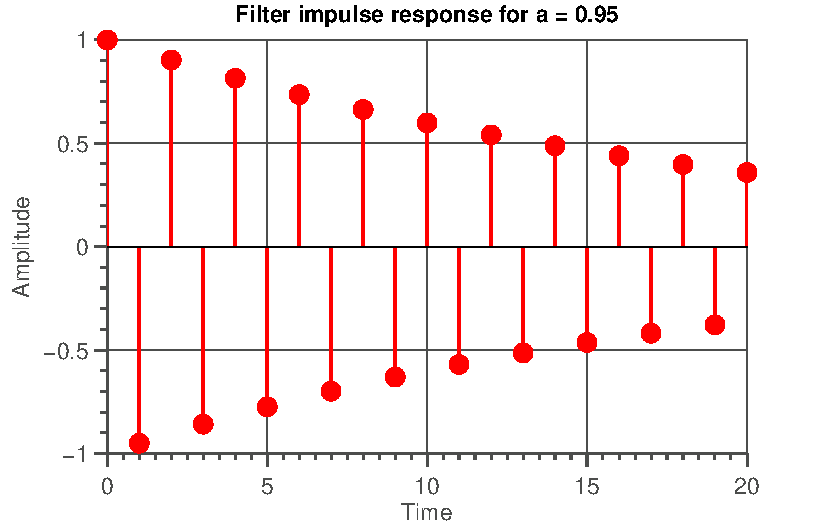
\includegraphics[width=\textwidth]{../../deliverable-7-resources/figures/ass-1/report-2/ass-1-report-2-a-positive.pdf}
	\end{subfigure}
	\begin{subfigure}{0.49\textwidth}
		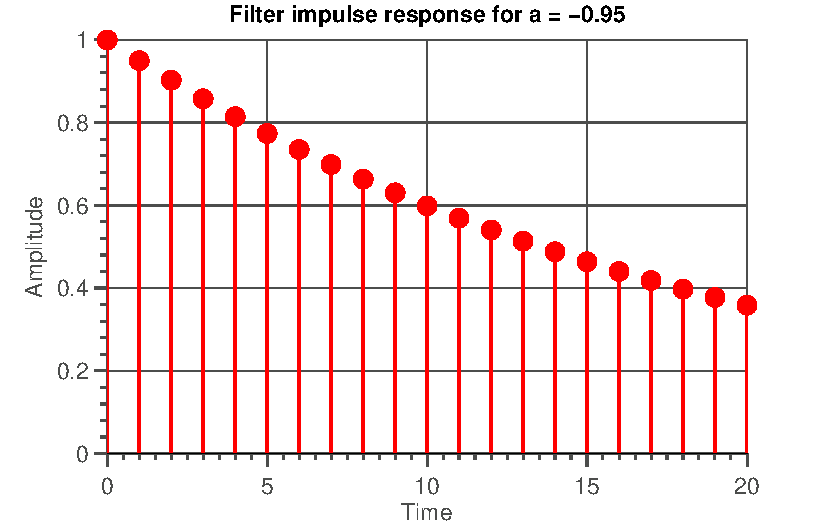
\includegraphics[width=\textwidth]{../../deliverable-7-resources/figures/ass-1/report-2/ass-1-report-2-a-negative.pdf}
	\end{subfigure}
	\caption{Impulse response of the given filter for two values of $a$}
	\label{fig:rep2-time-resp}
\end{figure}

The effect of this filer on more general signal can be described and explained as follows. ?????? 

To analyze the effect of this filter on signals frequency domain plots where plotted. The plots are displayed in figure Figure~\ref{fig:rep2-freq-resp} for $a=0.95$ and $a=-0.95$. Inspecting this impulse responces one can conclude that the filter behaves as a band-stop filter for $a=0.95$ and as a band-pass for $a=-0.95$. How this filter channges an impulse is ?????. For a more general signal it would mean ????. \\

\begin{figure}[H]
	\centering
	\begin{subfigure}{0.49\textwidth}
		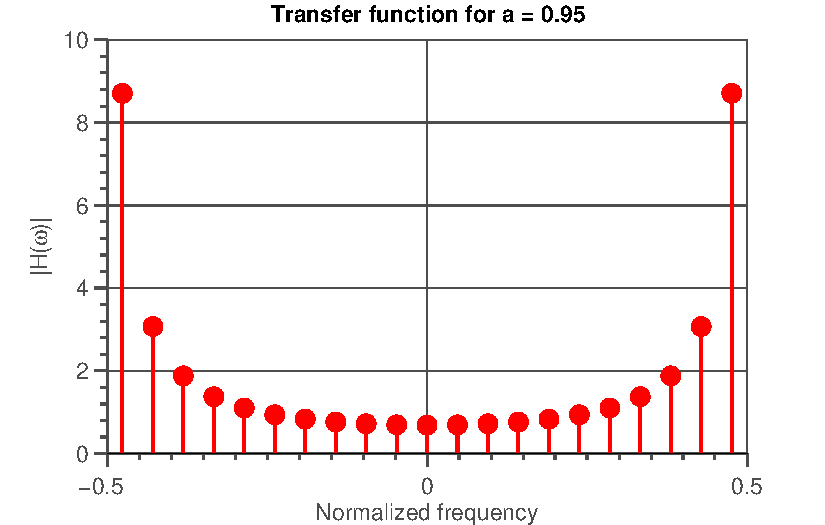
\includegraphics[width=\textwidth]{../../deliverable-7-resources/figures/ass-1/report-2/ass-1-report-2-a-positive-spectrum.pdf}
	\end{subfigure}
	\begin{subfigure}{0.49\textwidth}
		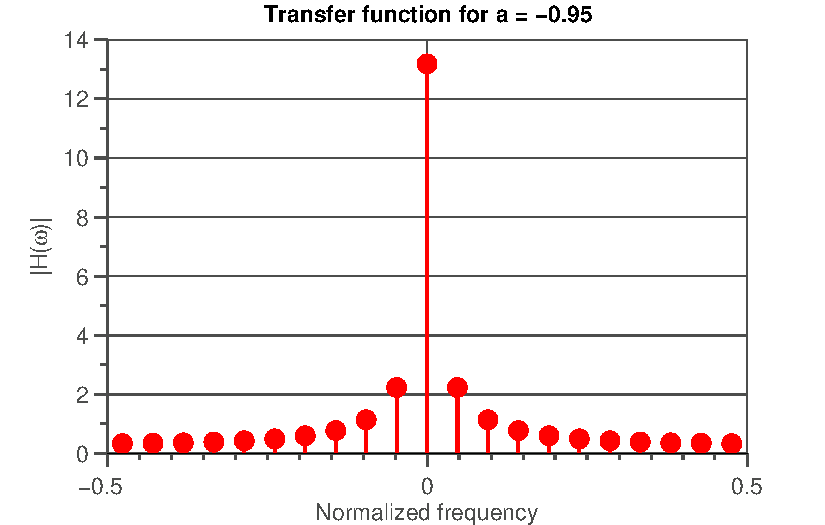
\includegraphics[width=\textwidth]{../../deliverable-7-resources/figures/ass-1/report-2/ass-1-report-2-a-negative-spectrum.pdf}
	\end{subfigure}
	\caption{The frequency response of the given filter for two values of $a$}
	\label{fig:rep2-freq-resp}
\end{figure}

Computers can't perform calculation on continious signals. And "FT" has a continious time input and continious frequency output. Also "DTFT" has a discrete time input and a continious frequency output. This is the reason why matlab has no build-in functions like "FT" and "DTFT". 

\subsection{Report 3}
In this report a signal called "train" will be analyzed. The time frequency plot is shown in figure Figure~\ref{fig:rep3-train-time}. 

%For this signal the frequency domain signal is also plotted in figure ?????.
%It can be seen that the frequency domain plot is symmetric around frequency$= 0Hz$. This symmetry exists because sine signals have the same form for negative and positive frequencies of the same value. In this case it makes sence to only take the positive frequencies since no extra information is added by the negative frequencies. This is done by deleting all information for frequencies under zero. 

\begin{figure}[H]
	\centering
	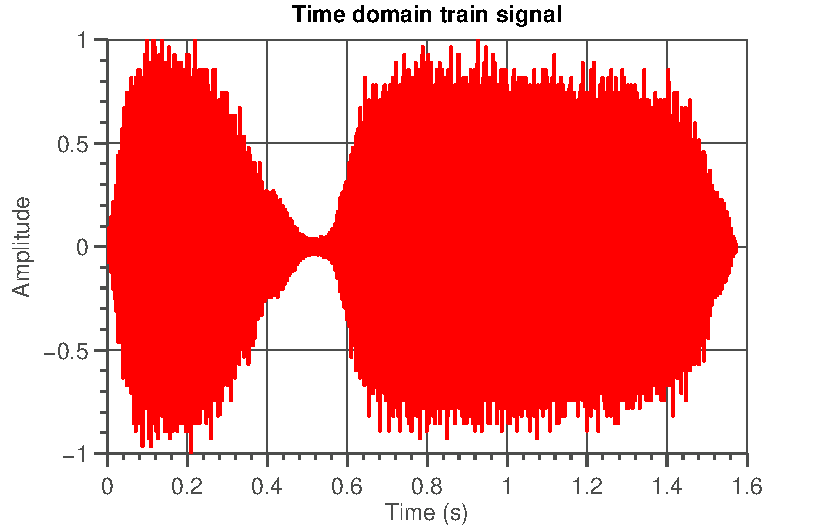
\includegraphics[width=0.6\textwidth]{../../deliverable-7-resources/figures/ass-1/report-3/ass-1-report-3.pdf}
	\caption{The time-domain signal of \texttt{MATLAB}'s train}
	\label{fig:rep3-train-time}
\end{figure}



\subsection{Report 4}
In Figure~\ref{fig:rep4-train-heatmap} a time-frequency plot of the train signal is displayed.

\begin{figure}[H]
	\centering
	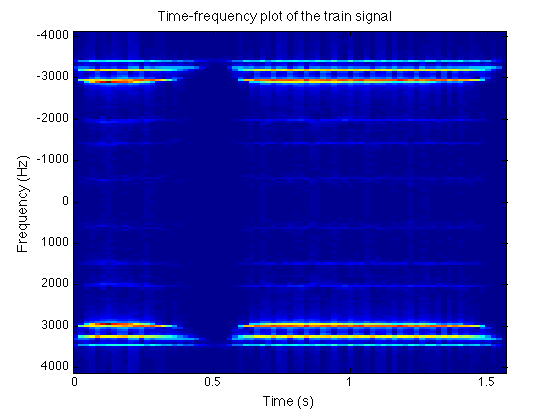
\includegraphics[width=0.6\textwidth]{../../deliverable-7-resources/figures/ass-1/report-4/ass-1-report-4.png}
	\caption{The frequency-time heatmap of \texttt{MATLAB}'s `train'}
	\label{fig:rep4-train-heatmap}
\end{figure}



\subsection{Report 5 and 6}

The purpose of this reports was to investigate what the influence is of zero padding. To do this we used the impulse response: $h[n]$ = [1  zeros(1,5)  0.9 zeros(1,5)  0.8]. 
The difference between the padded version and the original version can be seen when calculating the DFT of both signals. The frequency domain plot of both signals are therefore shown in Figure~\ref{fig:rep5-6-spectrum}. 
From this plot we see that every 5th sample in the padded response coincides with a sample of the original one. Thus we see that interpolation is achieved. Also we see that just by adding zeros one can enhance the DFT of a sequence. 

\begin{figure}[H]
	\centering
	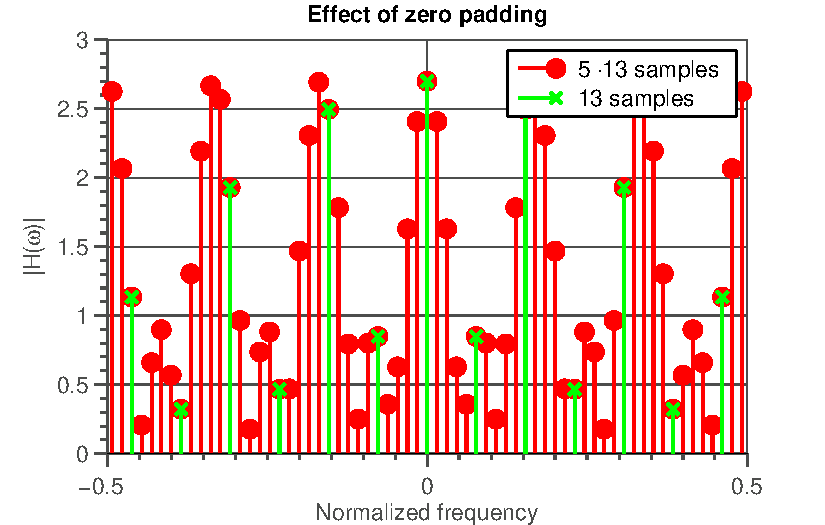
\includegraphics[width=0.6\textwidth]{../../deliverable-7-resources/figures/ass-1/report-5-6/ass-1-report-5-6.pdf}
	\caption{The frequency spectrum of the given signal $h$, with and without zero padding, obtained using FFT}
	\label{fig:rep5-6-spectrum}
\end{figure}


\subsection{Report 7}
Now we want to demonstrate the following convolution property: \newline

\begin{center}
 $y[n] = x[n]*h[n] \leftrightarrow Y(\omega) = X(\omega)H(\omega)$ 
\end{center}


Herein we assigned a 'train' sound to  $x[n]$.  And  $h[n]$ = [1  zeros(1,5)  0.9 zeros(1,5)  0.8].
In order to prove this property we want to show that the following equation is correct: \newline

\begin{equation}
\centering
 \mathcal{F}(y[n]) = X(\omega)H(\omega)
\end{equation}

First of all $y[n]$ was calculated by calculating the convolution of $x[n]$ and $h[n]$. From this convolution it follows that the length of sequence $y[n]$ is equal to $N = L + M - 1$, where $L$ is the length of $x[n]$ and $M$ the length of $h[n]$. This is why the length of $X(\omega)H(\omega)$ also has to be of legnth $N$. In order to achieve this $x_{0}[n]$ and $h_{0}[n]$ where created. $x_{0}[n]$ and $h_{0}$ are $x[n]$ and $h[n]$ respectively but with extra zeros until being both of length $N$. \\
After doing this the fourier transforms of $y[n]$, $x_{0}[n]$ and $h_{0}[n]$ where calculated. Finally the convolution property was demonstrated by plotting $Y(\omega)$ and $X(\omega)H(\omega)$. From the plots, shown in Figure~\ref{fig:rep7-convolution}, it  can be seen that the results are the same.

\begin{figure}[H]
	\centering
	\begin{subfigure}{0.49\textwidth}
		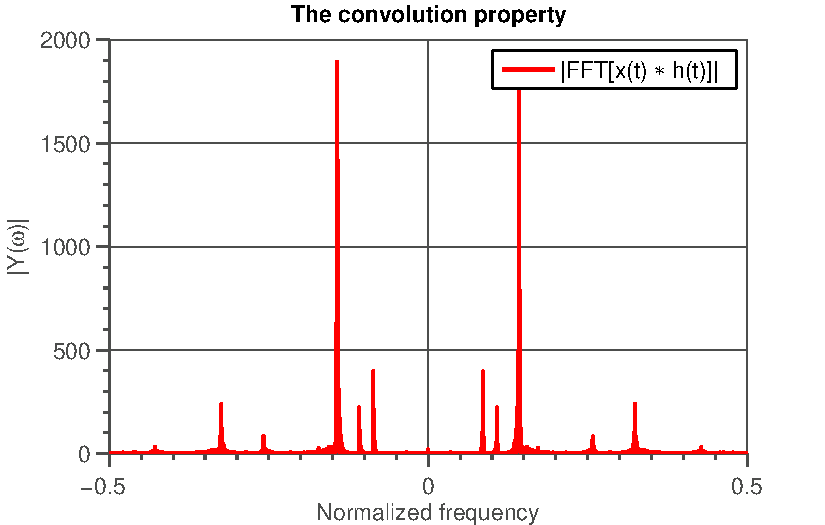
\includegraphics[width=\textwidth]{../../deliverable-7-resources/figures/ass-1/report-7/ass-1-report-7-convolution.pdf}
	\end{subfigure}
	\begin{subfigure}{0.49\textwidth}
		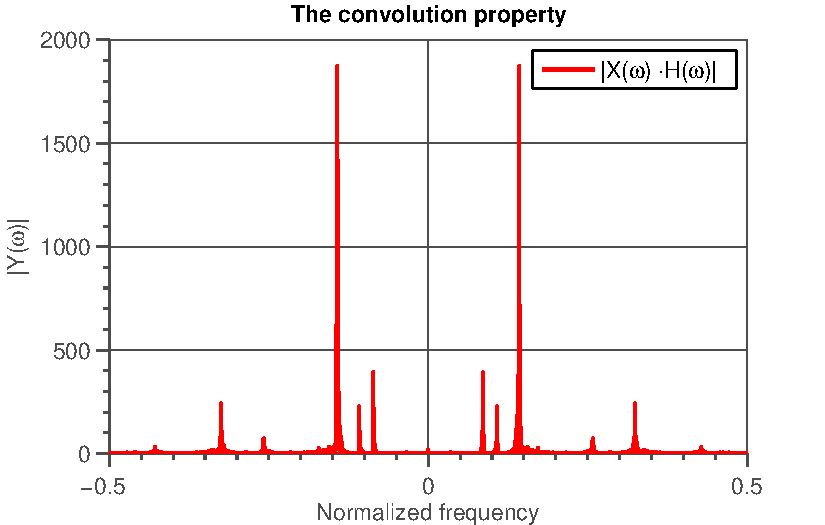
\includegraphics[width=\textwidth]{../../deliverable-7-resources/figures/ass-1/report-7/ass-1-report-7-multiplication.pdf}
	\end{subfigure}
	\caption{Comparison of spectra for testing the convolution property.}
	\label{fig:rep7-convolution}
\end{figure}






\end{document}